\section{Results and Analysis}



\subsection{Performance of FOLtR-ES on other dataset}

In the previous work, FOLtR-ES is conducted on MQ2007 and MQ2008 datasets~\cite{kharitonov2019federated}. To further study if the algorithm can achieve similar ranking performance on other publicly available LTR datasets. We perform experiments on MLSR-WEB10K dataset using same parameters chosen by~\cite{kharitonov2019federated}, using antithetic variates and setting $B = 4$ and $p = 0.9$. 

Unlike MQ2007 and MQ2008 datasets, FOLtR-ES performed on MLSR-WEB10K shows an opposite finding: the neural ranker dose not consistently perform better that the linear ranker. And for MLSR-WEB10K, FOLtR-ES takes more times on updating the ranker till it achieves the stable performance, which might be caused by larger training queries in MLSR-WEB10K. Figure \ref{fig: mslr-v0} shows the mean batch MaxRR of five data splits in MLSR-WEB10K with the three click models.

\begin{figure}[H]
	\centering
	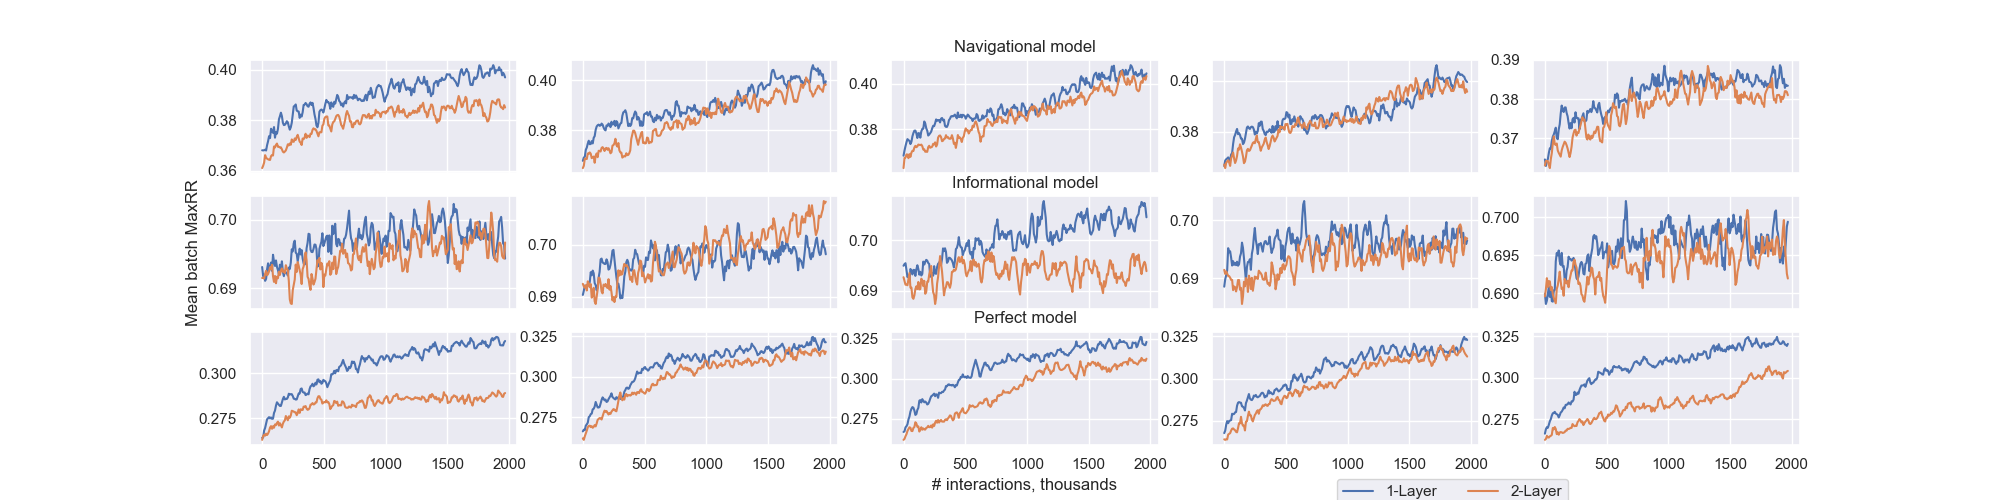
\includegraphics[width=16cm, height=5cm]{v0_mslr_foltr_per_batch.png}
	\caption{Mean batch MaxRR for MLSR-WEB10K with $p = 0.9$}
	\label{fig: mslr-v0}
\end{figure}


\subsection{Effects of number of clients on FOLtR-ES}
%To answer RQ1, we perform experiments on MLSR-WEB10K dataset with the same FOLtR-ES setup
%Reproducing FOLtR-ES on other datasets

To study the influence of number of clients, we perform experiments on MQ2007 and MSLR-WEB10K datasets. We vary the number of clients across {50, 1000, 2000} but set the fixed total updating times to 2000000 and set $B = 4$. We also set the privatization parameter $p$ across {0.5, 0.9, 1.0}.

Our experiments show that lower clients number will reduce the performance in the linear ranker. But for the neural ranker, the difference is minor.

\begin{figure}[H]
	\centering
	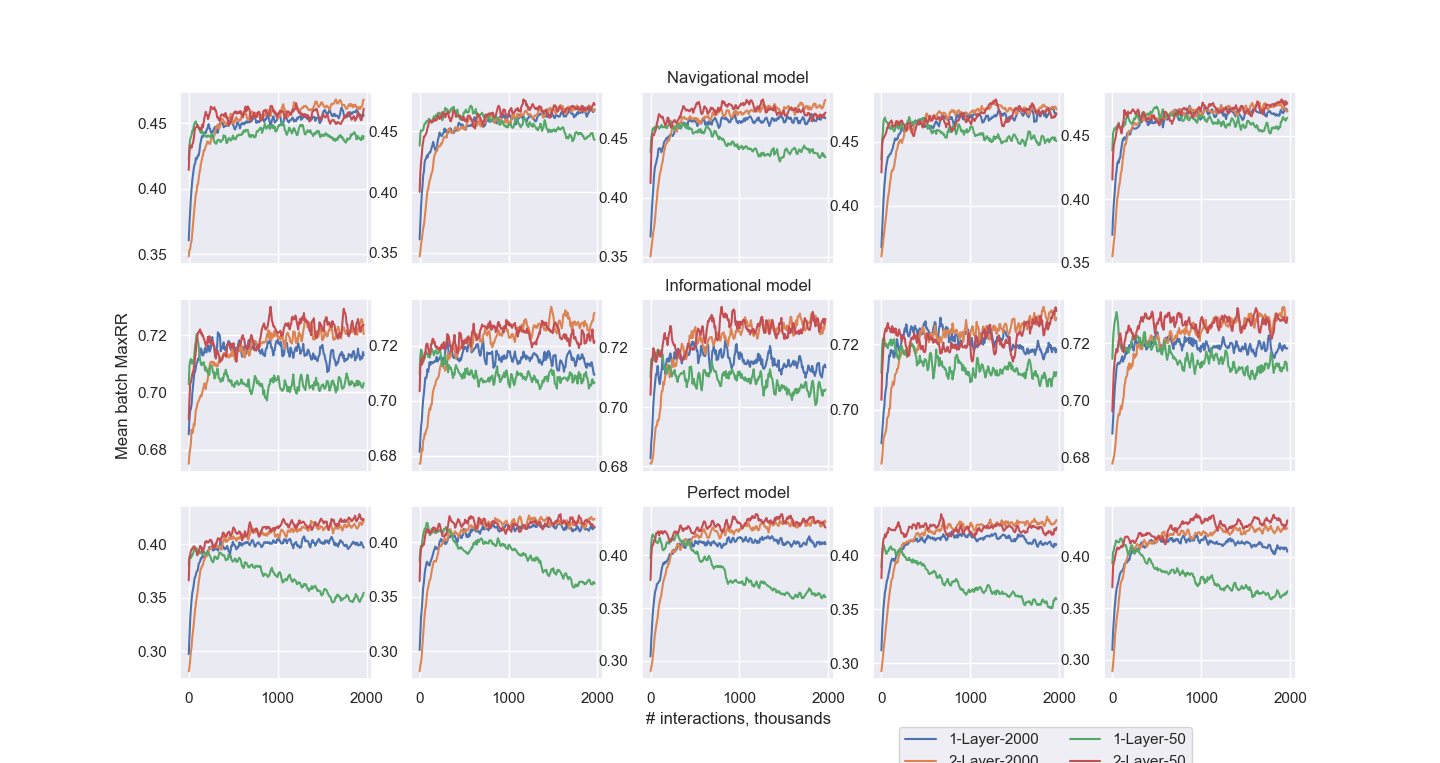
\includegraphics[width=16cm, height=8cm]{v0_mq2007_foltr_clients_p0.9.png}
	\caption{Mean batch MaxRR for MQ2007 with different client number}
	\label{fig: mq2007clients}
\end{figure}


\subsection{Comparing FOLtR-ES with OLTR baselines}

For a fair comparation, we set up the privacy probability $p = 1$ (lowest privacy) in FOLtR-ES. We perform experiments on MQ2007 and MLSR-WEB10K datasets with simulating 2000 clients.

\begin{figure}[H]
	\centering
	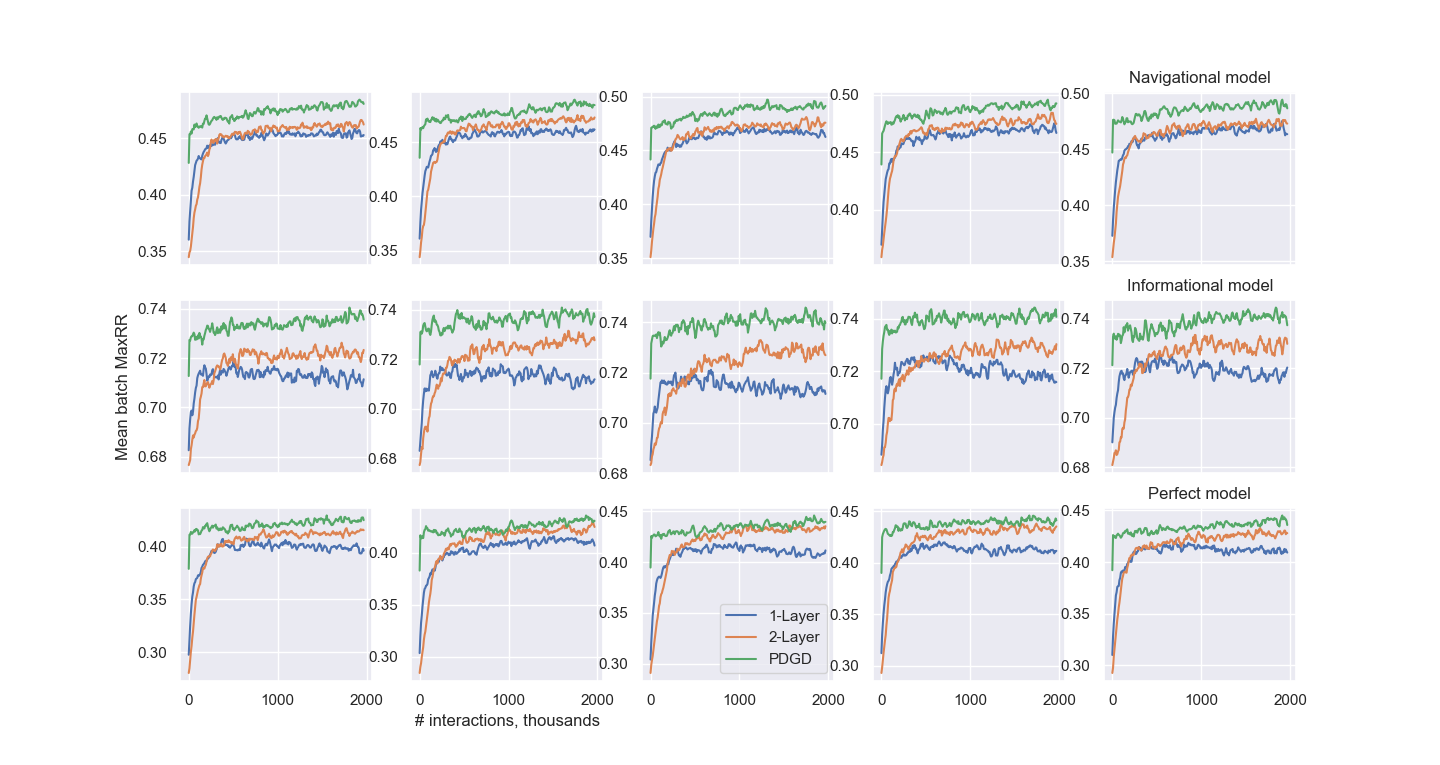
\includegraphics[width=16cm, height=8cm]{v0_mq2007_foltr_vs_pdgd_2000clients_p1.0.png}
	\caption{Mean batch MaxRR for MQ2007 with 2000 clients and $p = 1$}
	\label{fig: mq2007-v0-baseline}
\end{figure}

\begin{figure}[H]
	\centering
	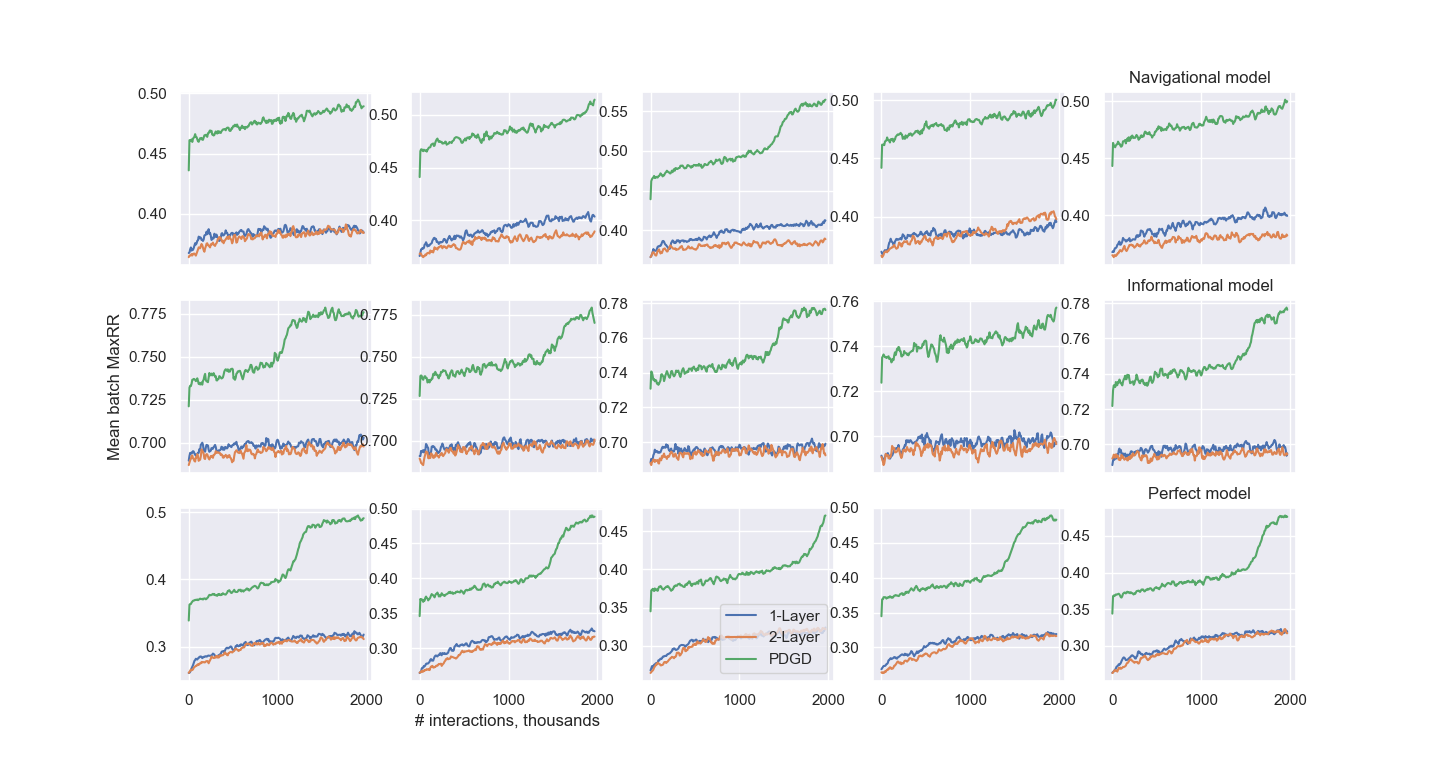
\includegraphics[width=16cm, height=8cm]{v0_mslr_foltr_vs_pdgd_2000clients_p1.0.png}
	\caption{Mean batch MaxRR for MSLR-WEB10K with 2000 clients and $p = 1$}
	\label{fig: mslr-v0-baseline}
\end{figure}

\subsection{Extending FOLtR-ES to other quality metric}



